\chapter{Implementation}

Differential GPS was evaluated as a suitable method to enhance the GPS position accuracy to the required level of 1 meter RMS.
This chapter documents the proccess of implementing it as a proof of concept.
Although this project is not planned to be used in this years competition, the system is designed to work with the current hardware of project TELL.
Section \ref{sec:tell_infrastructure} shows what is already implemented in project TELL.
How DGPS can be integrated into this infrastructure is explained from section \ref{sec:system_overview} onward.


\section{TELL Organization and Infrastructure}\label{sec:tell_infrastructure}

At the time of writing, the rocket of prject TELL is being made ready to ship to the U.S. for the 2018 Spaceport America Cup.
The whole project is divided into the 7 subteams: Simulations, Structures, Propulsion, Avionics, Control, and Recovery.
This bacelor thesis is a project of the Avionics subteam.
The Avionics subteam is responsible for the sensor data aquisition which used by the controll and for logging, as well as a telemetry link to a ground station to transmit the most important metrics to monitor the flight performance and recover the rocket.
Apart from the rocket called TELL \rom{1}, the hardware consists of a ground station with laptop, telemetry link, and GPS reference station.

\subsection{The Rocket}

TELL \rom{1} is the vehicle that shall propel the 4 kg payload to the target apogee of 10'000 feet (3048 meters) at the competition.
In figure \ref{fig:tell_1} it is shown in the wind tunnel test.
It has a length of 2.42 meters, weights 24 kg at liftoff, and is porpelled by a solid motor with an average thrust of 2245 N.
With those parameters, the rocket is designed to overshoot the target apogee.
Air brakes driven by a controll loop are used to correct the apogee.

\begin{figure}[ht]
 \centering
 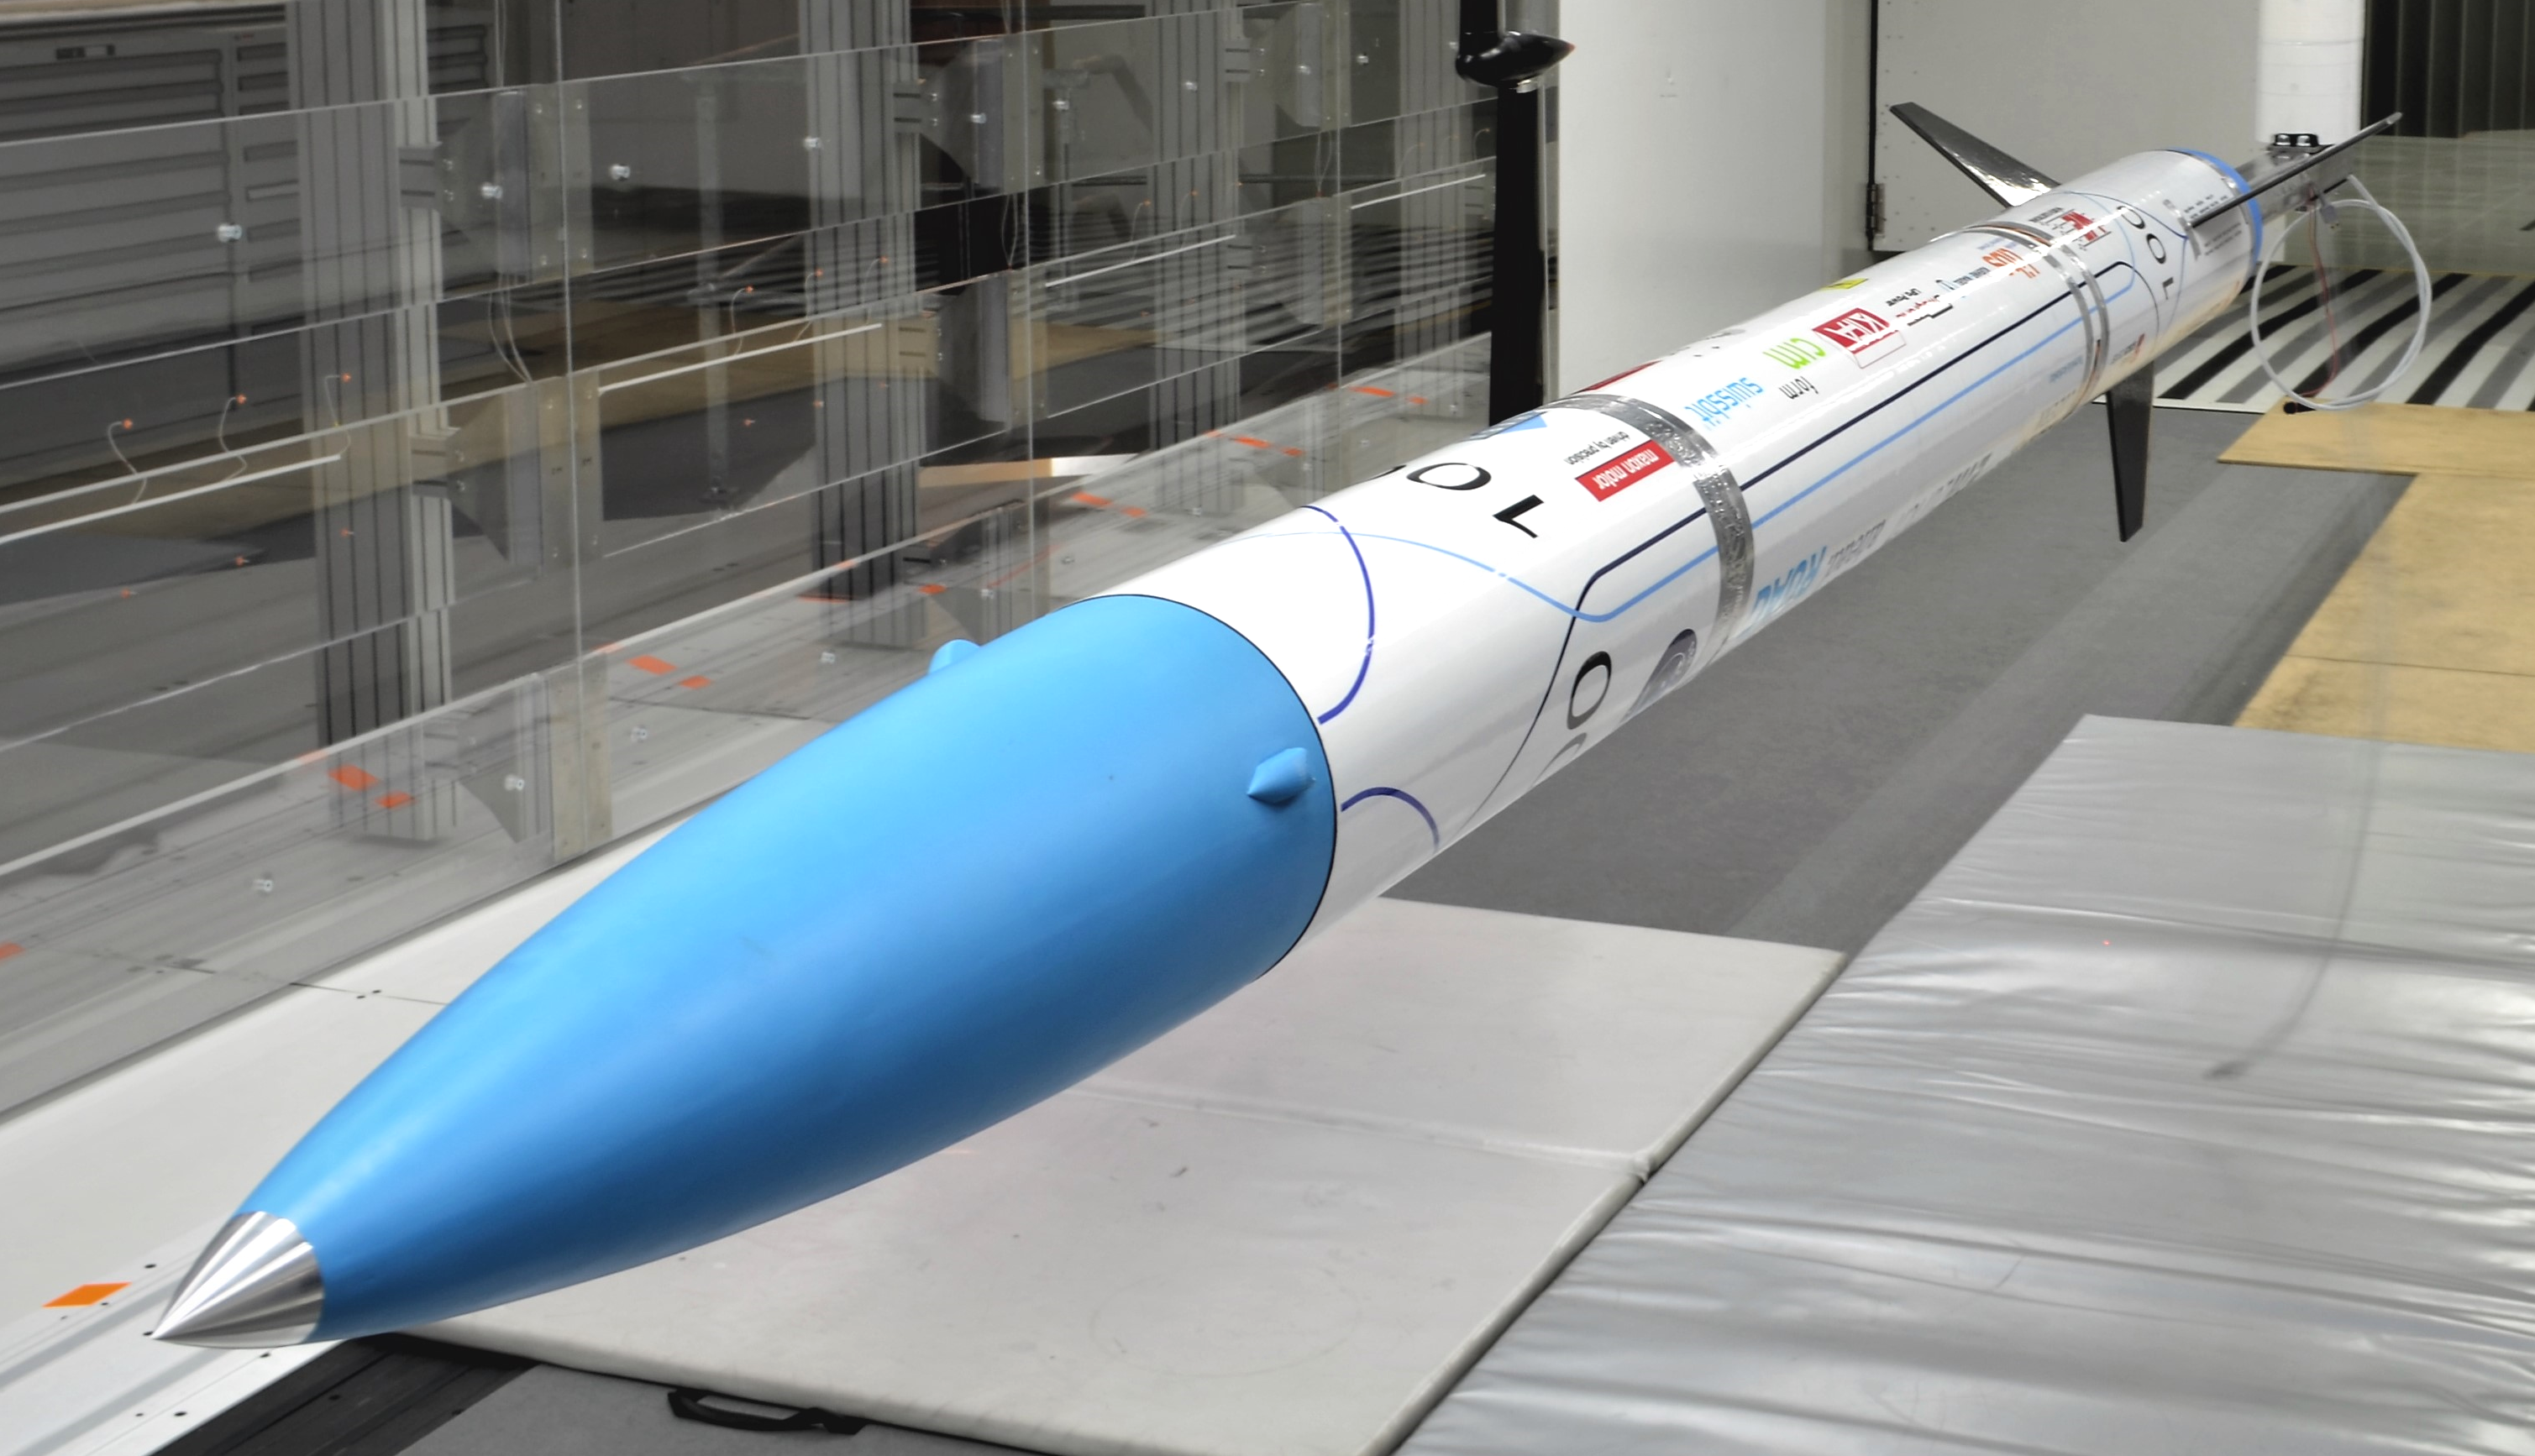
\includegraphics[height=6cm]{images/TELL_1.png}
 \caption{TELL \rom{1} in the wind tunnel}
 \label{fig:tell_1}
\end{figure}

The avionics on the rocket are split into the two parts nasecone avionics and lower body avionics as shown in figure \ref{fig:tell_structure}.
Both parts are the same appart from the GPS and telemetry in the nosecone, and two additional barometers, rocket motor temperature sensor and payload interface for the lower body avionics.
Sensors that both parts have separately are an acceleromert, magnetometer, gyroscope and climate sensor.
Both parts also log their collected data to a seperate SD card.
This is done to have redundancy and to be able to have sensors in all parts of the rocket.
The two parts are connected over a wireless link to be able to communicate after the nosecone is popend off at the first recovery event.
The central component of each avionics module is an ARM M4 microcontroller that acts as the flight controller.
It connects to all the sensors and communication modules of its half of the rocket.

The nosecone avionics has two GPS antennas with a separate receiver for each.
One is directed upwards to have reception in the time from launch to the apogee.
The other is directed downwards to have reception after the nosecone is hanging upside down after the first recovery event.
The telemetry transmitter and antenna are also implemented in the nosecone.
As the transmitter, the XBee-PRO SX module is used.
It transmitts on the frequency band from 902 to 928 MHz, which is open for public use in north america, where the competition is taking place.
With a transmitting power of 1 W, it can establish a link over a range of up to 105 km.

\begin{figure}[ht]
 \centering
 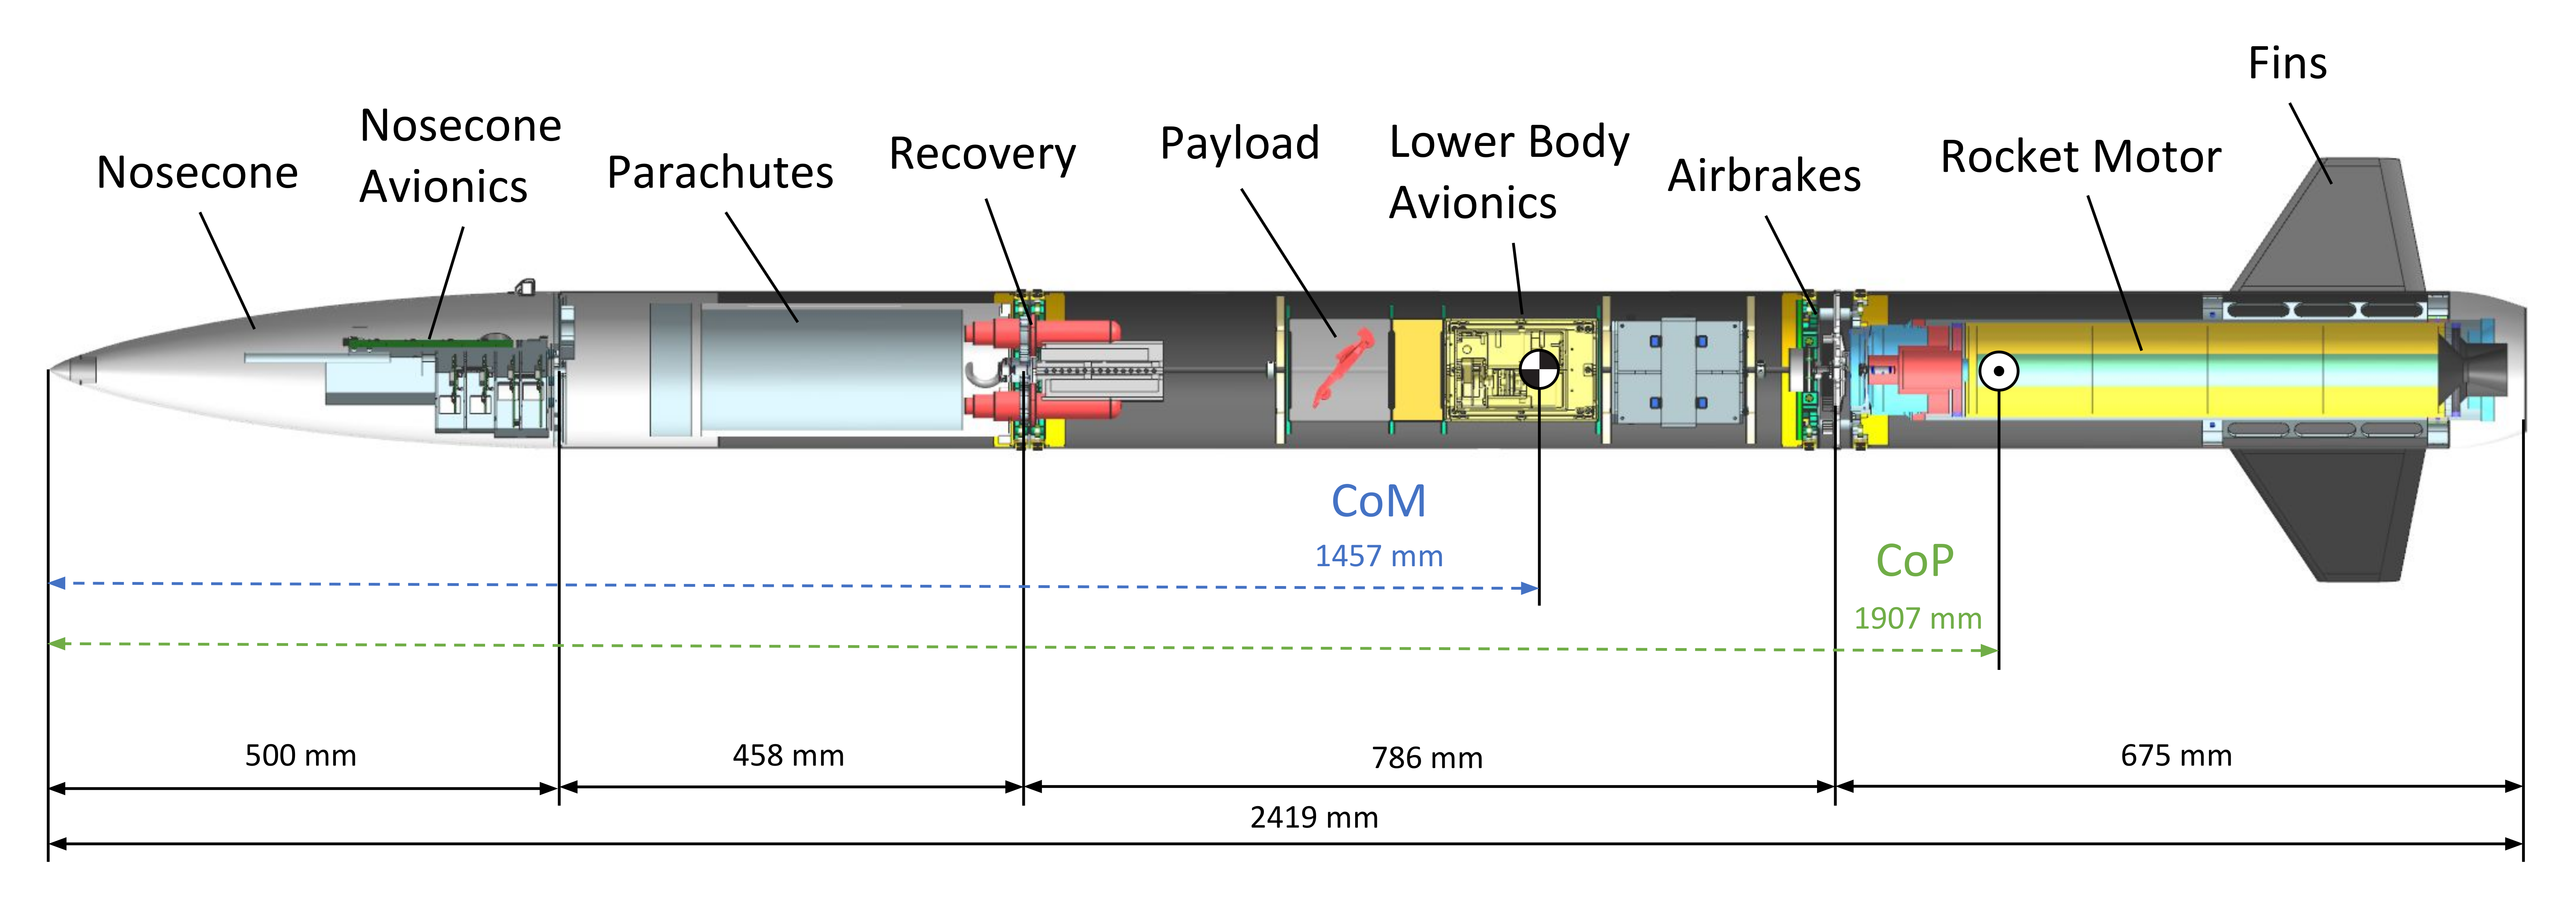
\includegraphics[width=\textwidth]{images/TELL_Structure.png}
 \caption{Overview of TELL}
 \label{fig:tell_structure}
\end{figure}

\subsection{The Ground Station}

The central part of the ground station is the a laptop that displays the live flight metrics.
Connected to it over USB is a second XBee module, that receives the telemetry data sent by the rocket.
A directional antenna is used to receive the downstream.

In this years project, it is planned to do post-processing DGPS to analize the trajectory.
GPS raw data has to be logged on the rocket and at a reference station in order to do that.
For post-processing DGPS, no data link is needed to the rocket.
A GPS receiver is placed at the ground station to act as the reference station.
The GPS module M8T fron u-blox was choosen for this purpose and is used in the rockets nosecone avionics, as well as at the ground station.
The speciality of the M8T module is, that it provides raw GPS data like the measured pseudoranges.
This is needed for post-processing DGPS.


\section{System Overview}\label{sec:system_overview}

The difference of the DGPS system described in this thesis to the post-processing one used by project TELL is when the corrected position is availabel.
A real-time system is needed that the corrected position can be directly used to controll the rocket.
This adds the requirement for a live PRC calculation, a data link to the rocket, and the inclusion of the corrections into the position estimation on the rocket.

Let's start with the data link.
Is is needed to send the corrections from the reference station, which is in this case the ground station, to the rocket.
With the telemetry system, a link is already established.
Although this is only a downlink for project TELL, the used XBee modules can be configured for a two way communication link.

For the DGPS to work, the measured pseudoranges on the rocket have to be corrected with the PRCs before they are used to estimate the position.
There are two possible ways to achieve this.
For the first way, the receiver would have to provide raw GPS data to the flight computer where the PRC can be added.
The position would then have to be estimated outside the receiver by the flight computer.
The challenge with this approach is, that the implementation of a position estimation algorithm from raw GPS data is huge development effort, especially on a microcontroller.
The second way is to choose a GPS receiver that accepts PRCs in a certain format and includes them in its position estimation.
This method has the advantage of a much smaller development effort because the position estimation can be left to the receiver.
The drawback is that the specific DGPS protocol accepted by the receiver has to be used, which limits the design freedom.
Both methos are possible with the current M8T GPS receiver.
It was specifically choosen because it outputs raw GPS data like the pseudoranges.
It also accepts PRCs in the form of a RTCM data stream, which is described in setion \ref{sec:rtcm}.
The second approach, where the receiver estimates the position, was choosen for this project to make it feasible to implement the system.
There are other receivers besides the M8T that have this functionality.
The selection of the receiver is addressend in section \ref{sec:receiver}.

Finally, the PRCs have to be generated at the ground station.
A similar trade off between flexibility and small development effort as for the position estimation in the rocket has to be made here.
The PRCs can either be calculated from GPS raw data, or a receiver with integrated reference station functionality can be used.
The decision was made in favor of a custom reference station algorithm.
The development effort is not as big as for a position estimation algorithm.
Also, such a system can more easily be impelemented in parallel to the current post-processing DGPS method, which will always be more precise than a real-time solution for post-flight analysis.
The custom application developed to generate the PRCs is described in section \ref{sec:dgps_message_generator}.

\begin{figure}[ht]
 \centering
 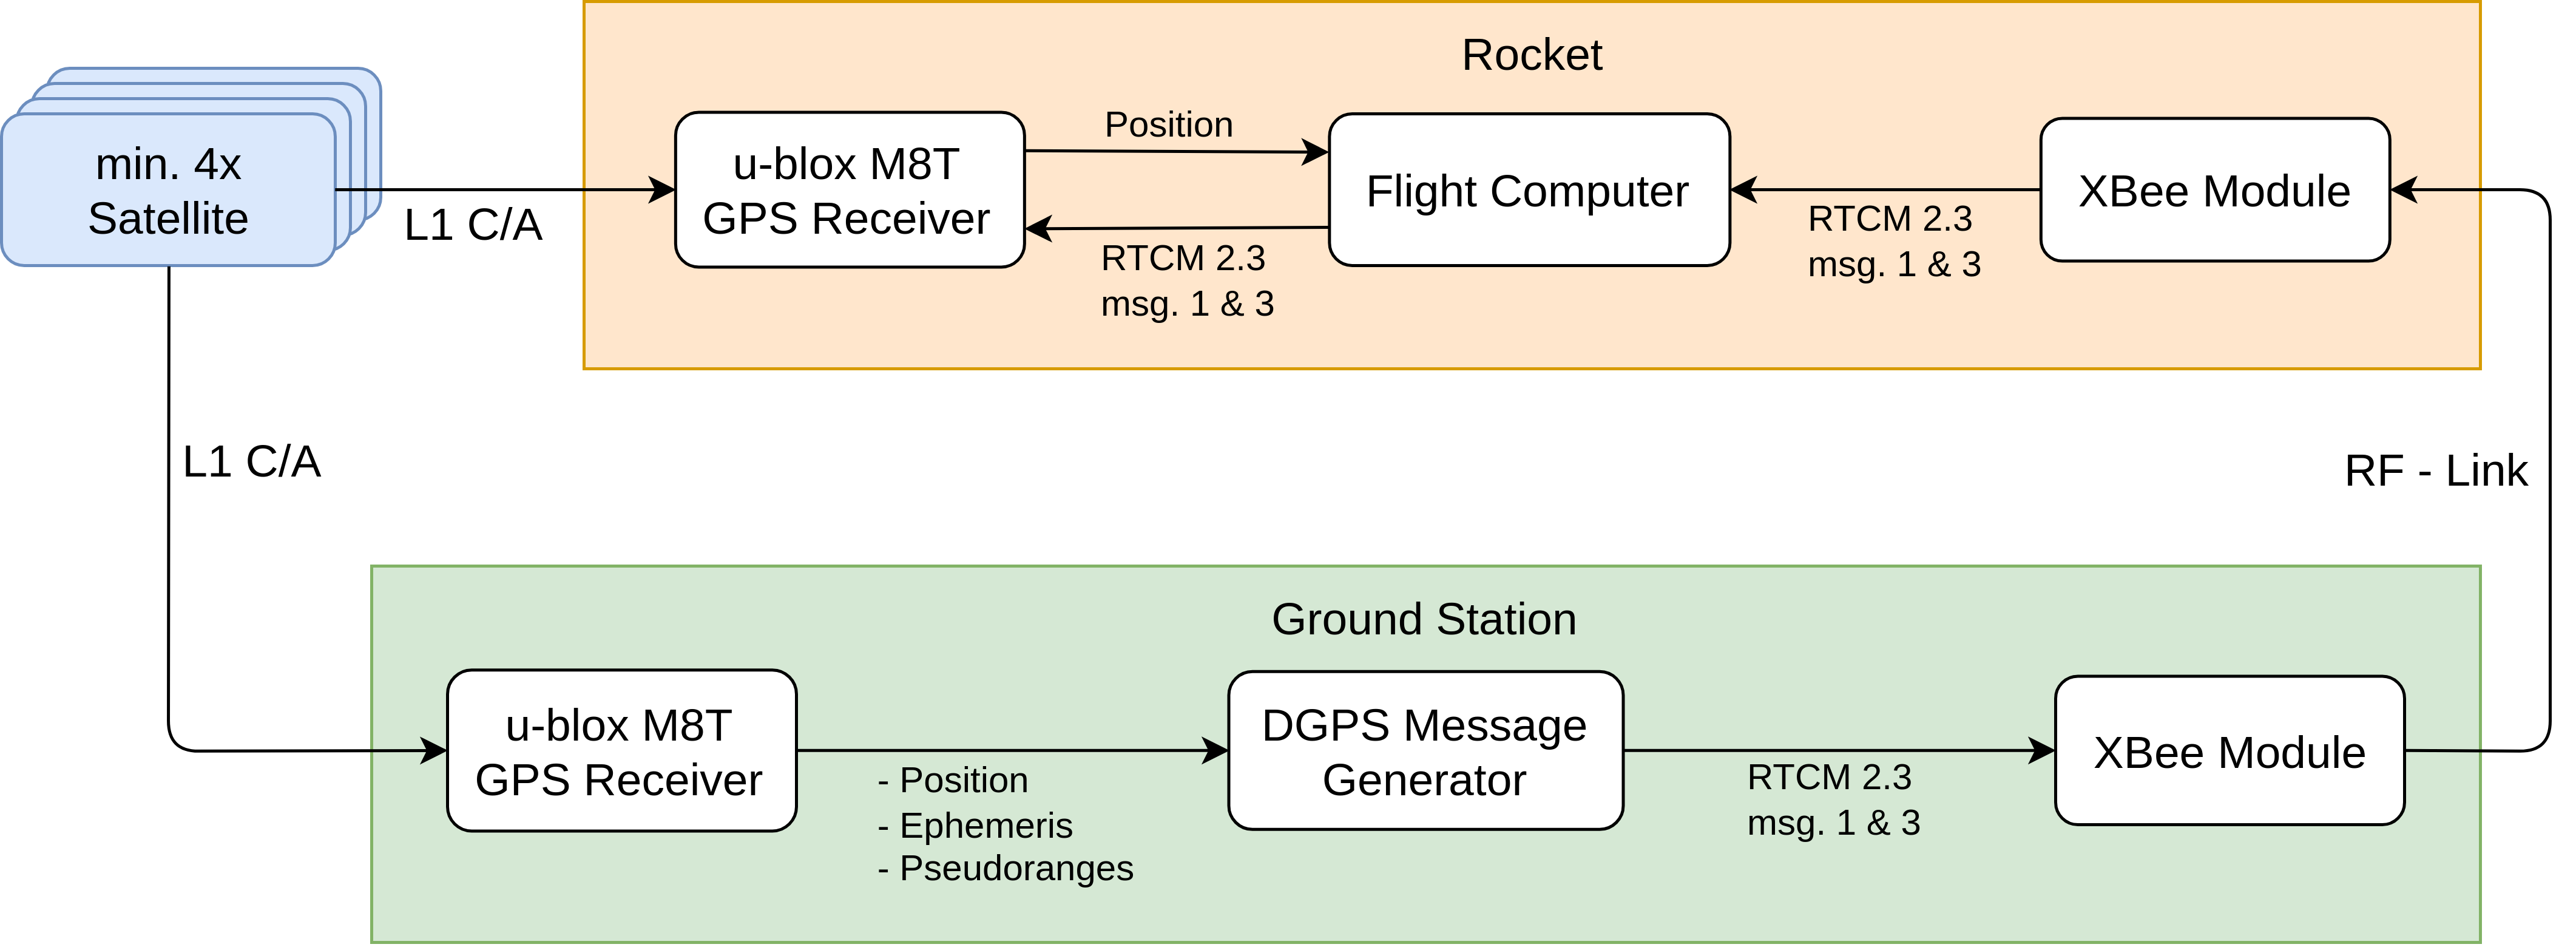
\includegraphics[width=\textwidth]{images/DGPS_System_Overview.png}
 \caption{DPGS data flow}
 \label{fig:data_flow}
\end{figure}

A top level view of the data flow for the planned system is shown in figure \ref{fig:data_flow}.
It starts with the generation of the GPS signals by the satellites.
The standard L1 C/A signals are used.
Both receiver have to receive the signals from a set of at least four satellites for the system to work.
The receiver at the ground station then measures the pseudoranges, decodes the navigation messages, and estimates its position.
It then sends its position, the navigation message bits which include the ephemeris data, and the measured pseudoranges to the ground station laptop over a USB connection.
This data is processed by the custom DGPS message generator application running on the ground station laptop.
The calculated PRCs are packed in messages of the RTCM 2.3 standard.
Message 1 and 3 of the standard are needed by the M8T receiver.
They are sent over another USB connection to the XBee module of the ground station to be transmitted over the RF link to the rocket.
The messages are forwarded to the flight computer in the nosecone, where they are separated from other data and fed into the GPS receiver on the rocket.
This receiver then corrects its pseudoranges with the latest PRCs before estimating the rocket position.


\section{GPS Receiver}\label{sec:receiver}

\begin{minipage}{0.6\textwidth}
  A seen in figure \ref{fig:data_flow}, the M8T receiver from u-blox used by TELL was also choosen for this project.
  The reasons for this decision were the following:
  \begin{itemize}
  \item output of raw GPS data
  \item support of the RTCM 2.3 standard
  \item same receiver can be used for rocket and reference station
  \item compatibility with post-processing DGPS
  \end{itemize}
  The avionics of project TELL are modular with separate boards for telemitry, GPS, and intra-rocket communication.
  This reduces the development effort and faulty parts can be replaced more easily.
  The different boards are connected with RS232 interfaces.
  Figure \ref{fig:m8t_receiver_board} shows the GPS board with a M8T receiver, antenna connector, RS232 interface, USB interface, and 12 V input.
  This board is used twice in the rocket and once at the ground station as post-processing DGPS reference station for project TELL.
  The exact same hardware setup can be used for the real-time DGPS.
\end{minipage}
\hfill
\begin{minipage}{0.37\textwidth}
 \centering
 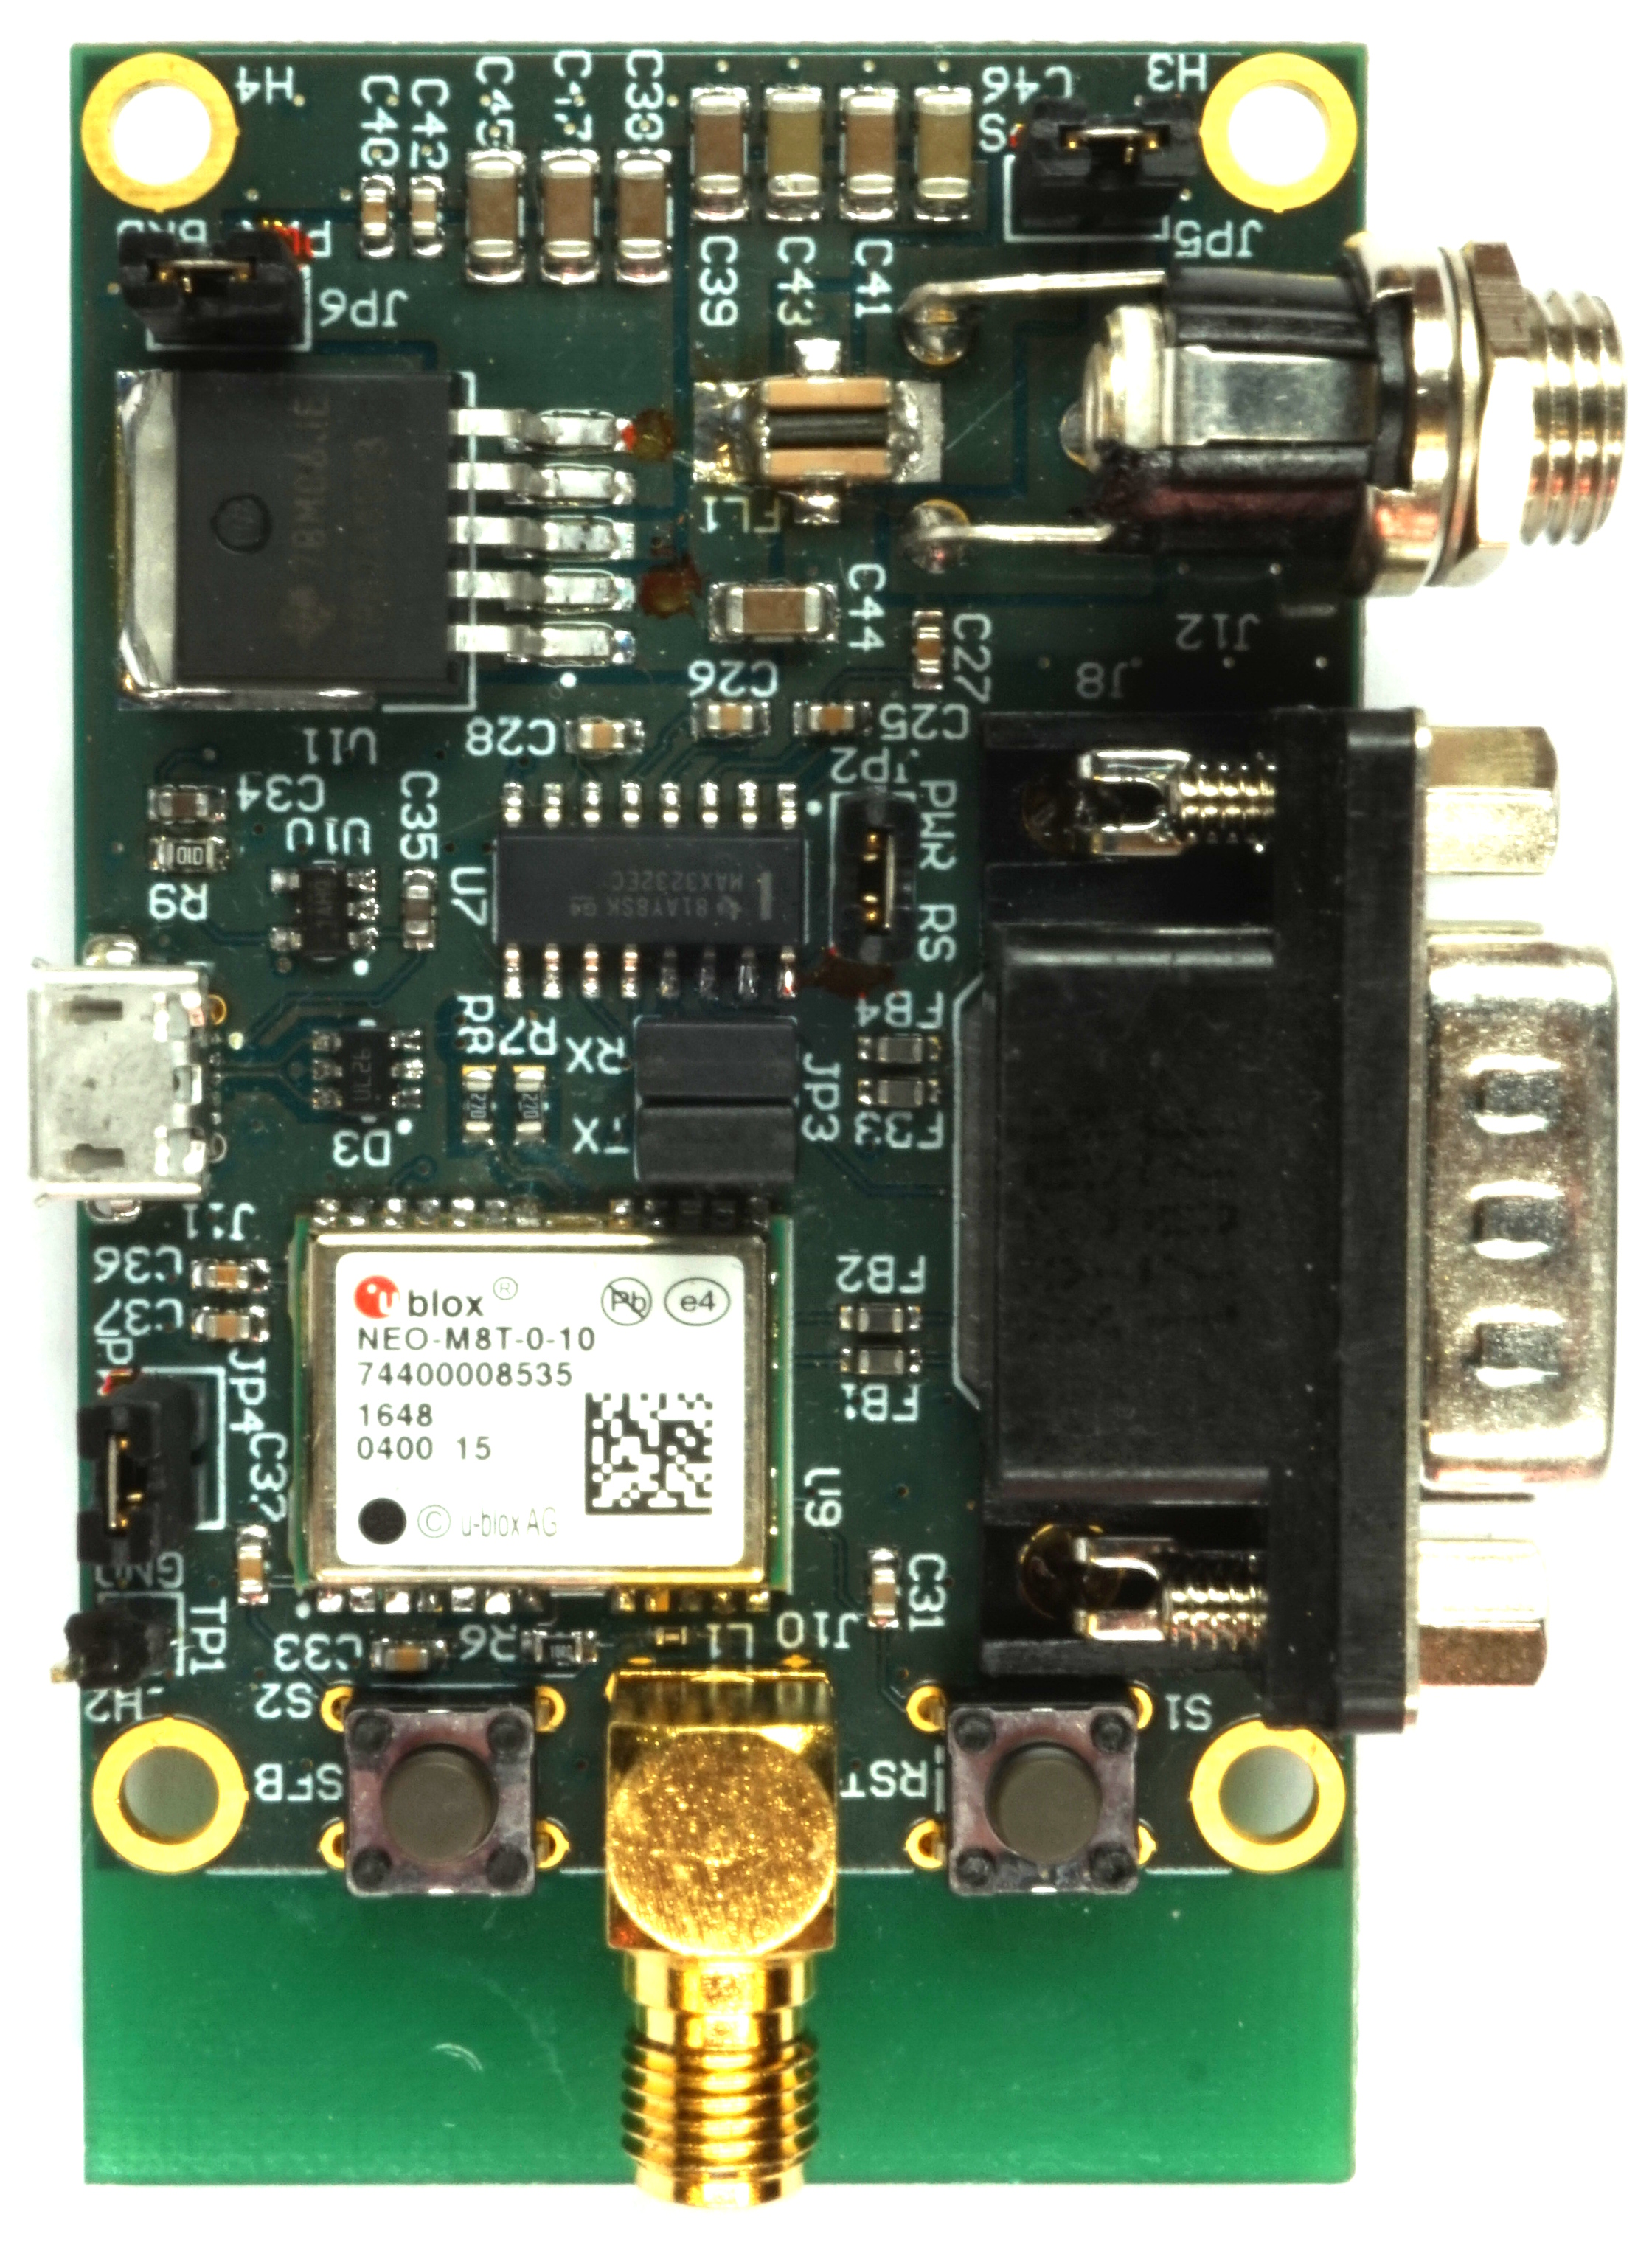
\includegraphics[width=\textwidth]{images/M8T_Receiver_Board.jpg}
 \captionof{figure}{GPS board of project TELL with u-blox M8T receiver}
 \label{fig:m8t_receiver_board}
\end{minipage}

GPS receivers from u-blox can communicate with messages from three different protocols.
The first one being NMEA.
It the standard way for GPS receivers to output their data.
It is in ASCII format which makes it easy to find in a bit stream.
All the standard data like time, position and satellite information can be aquired with NMEA messages.
The second is the u-blox proprietary UBX protocol.
Much more specific information can be optained with UBX messages like the GPS raw data in the case of the M8T receiver.
It is also use to configure the receiver.
The third protocol understand by u-blox receivers is RTCM.
This is a set of standards for receiver independent differental GPS corrections.
It is described in section \ref{sec:rtcm}.

A requirement for the receiver on the rocket is that the acceleration, velocity and altitude experienced on a sounding rocket do not exceede its operational limits.
The operational limits of 50'000 meters max. altitude and 500 m/s max velocity of the M8T receiver are both sufficient.
The goal of the competition is to go to an altitude of 3048 meters.
The max. speed reached by TELL will be at the border of supersonic which is 343 m/s.
Those are legal limits where the receiver must not provide a fix if exceeded.
The acceleration limit on the other hand is caused by the implementation of the receiver.
It is only 4 g, whereas TELL will experience up to 10 g of acceleration.
This could pose a problem.
But the receiver is actually not required to get a fix during the burn when the acceleration is experienced.
It only has to get a fix max. 2 seconds after burnout.
If the reaquisition time is sufficiently small, the receiver could still meet the requirements.
This parameter is not given in the datasheet, but the related parameter of a time-to-first-fix in case of a hot start is given as 1 second.
If this requirement will be met can only be definitively confirmed with a rocket flight test. \cite{M8T}


\section{RTCM 2.3 Standard}\label{sec:rtcm}

RTCM stands for Radio Technical Commission for Maritime Services.
It is an organization that defines standards mainly for use in matitime applications.
One group of standards define the protocol for DGPS corrections.
There are three generations of standards in this group.
The most recent ones being 10403.3 of the third generation and 10402.3 of the second generation.
U-blox GPS receivers with the possibility of DGPS understand either of those standards.
In the case of the M8T it is 10402.3 which is mostly just called RTCM 2.3 \cite{RTCM_2.3}.

The RTCM 2.3 standard defines 30 messages.
The messages are divided into 30 bit long words like the GPS navigation messages.
The last 6 bits of each word are parity bits.
The parity algorithm is also adopted form the GPS navigation messages and can be found in the GPS Interface Specification \cite{IS-GPS-200}.
It defines that the parity of each word is connected to the last two parity bits of the previous word.
This is also true across messages for the RTCM 2.3 standard.
Each message starts with a header of two words that includes a preamble, the message type, the station I.D., a modified verson of the z-count (time reference in navigation messages), a sequence number, the number of data words in this message, and the station health.

The M8T receiver requires message 1 and message 3 to enter DGPS mode.
Message 1 is used to transmit the DGPS corrections.
For each satellite a PRC is calculated, this message transmits a scale factor, user differential range error (UDRE), pseudorange correction, range-rate correction, and issue of data (IOD).
The scale factor determines the scale of the pseudorange correction to 0.02 or 0.32 m and the range-rate correction to 0.002 or 0.032 m/s.
The UDRE is the estimated error in the differental corrections.
The range-rate corrections can be used to interpolate between pseudorange corrections.
It is no longer necessary since Selective Availability (a intended noise introduced to civil GPS signals) was switched off in the year 2000 and can be set to 0.
The IOD is sent to ensure that both the refernce station and the user use the same parameters to calculate the satellite position.
Message three transmits the XYZ coordinates of the reference station in the WGS 84 reference frame.
This message is needed to determined the closest reference station if multiple RTCM streams are received.

It is important for the system to work that both the reference station and the user correct the pseudoranges for the same errors.
The standard states that the raw pseudoranges have to be adjusted for the receiver clock offset, satellite clock offset, satellite relativistic corrections, and L1-L2 group delay correction in the case of a dual frequency receiver.
Neither of the atmospheric errors should be modeled to correct the pseudoranges.
Only a tropospheric model that incorporates the different altitudes of the reference station and user can be applied if necessary.
For the data link, an update rate of once every 30-60 seconds is stated as adequate.


\section{DGPS Message Generator}\label{sec:dgps_message_generator}

It was decided to develop a custom application to generate the PRCs from the raw GPS data at the reference station.
This made up the biggest part of the development effort for this project.
The application has to run on the ground station laptop and connect to the GPS receiver as input and the XBee module as output.
It was written in C++ and developed to run on Linux.
For the development environment, Qt Creator was choosen.

\newpage

\subsection{Software Architecture}

The different files of the application and their connections are shown in figure \ref{fig:software_architecture}.
On application startup, the MainWindow widget starts running.
It is responsible for the graphical user interface (GUI) and the start of the underlying programs.
Before the DGPSMesGen can be started, the application has to know the location of the reference station.
This position can either measured with the PositionAveraging, or it can be loaded from a file or from the RefPosDialog.
When the reference position is set, the DGPSMesGen can be started.
It then starts the UBloxInterface, XBeeInterface and NavMessageDecoder.
The DGPSMesGen and the three newly started threads communicate over multiple instances from the ThreadQueue class.
The data types used to transmit data over the ThreadQueues are defined in the header files GPSDataTypes and UBloxMessages.
Additional functions used by the UBloxInterface and XBeeInterface are implemented in the files TypeConversion and RTCMEncode.
A Debug header file is used to enable debug, and logging functionality.

\begin{figure}[ht]
 \centering
 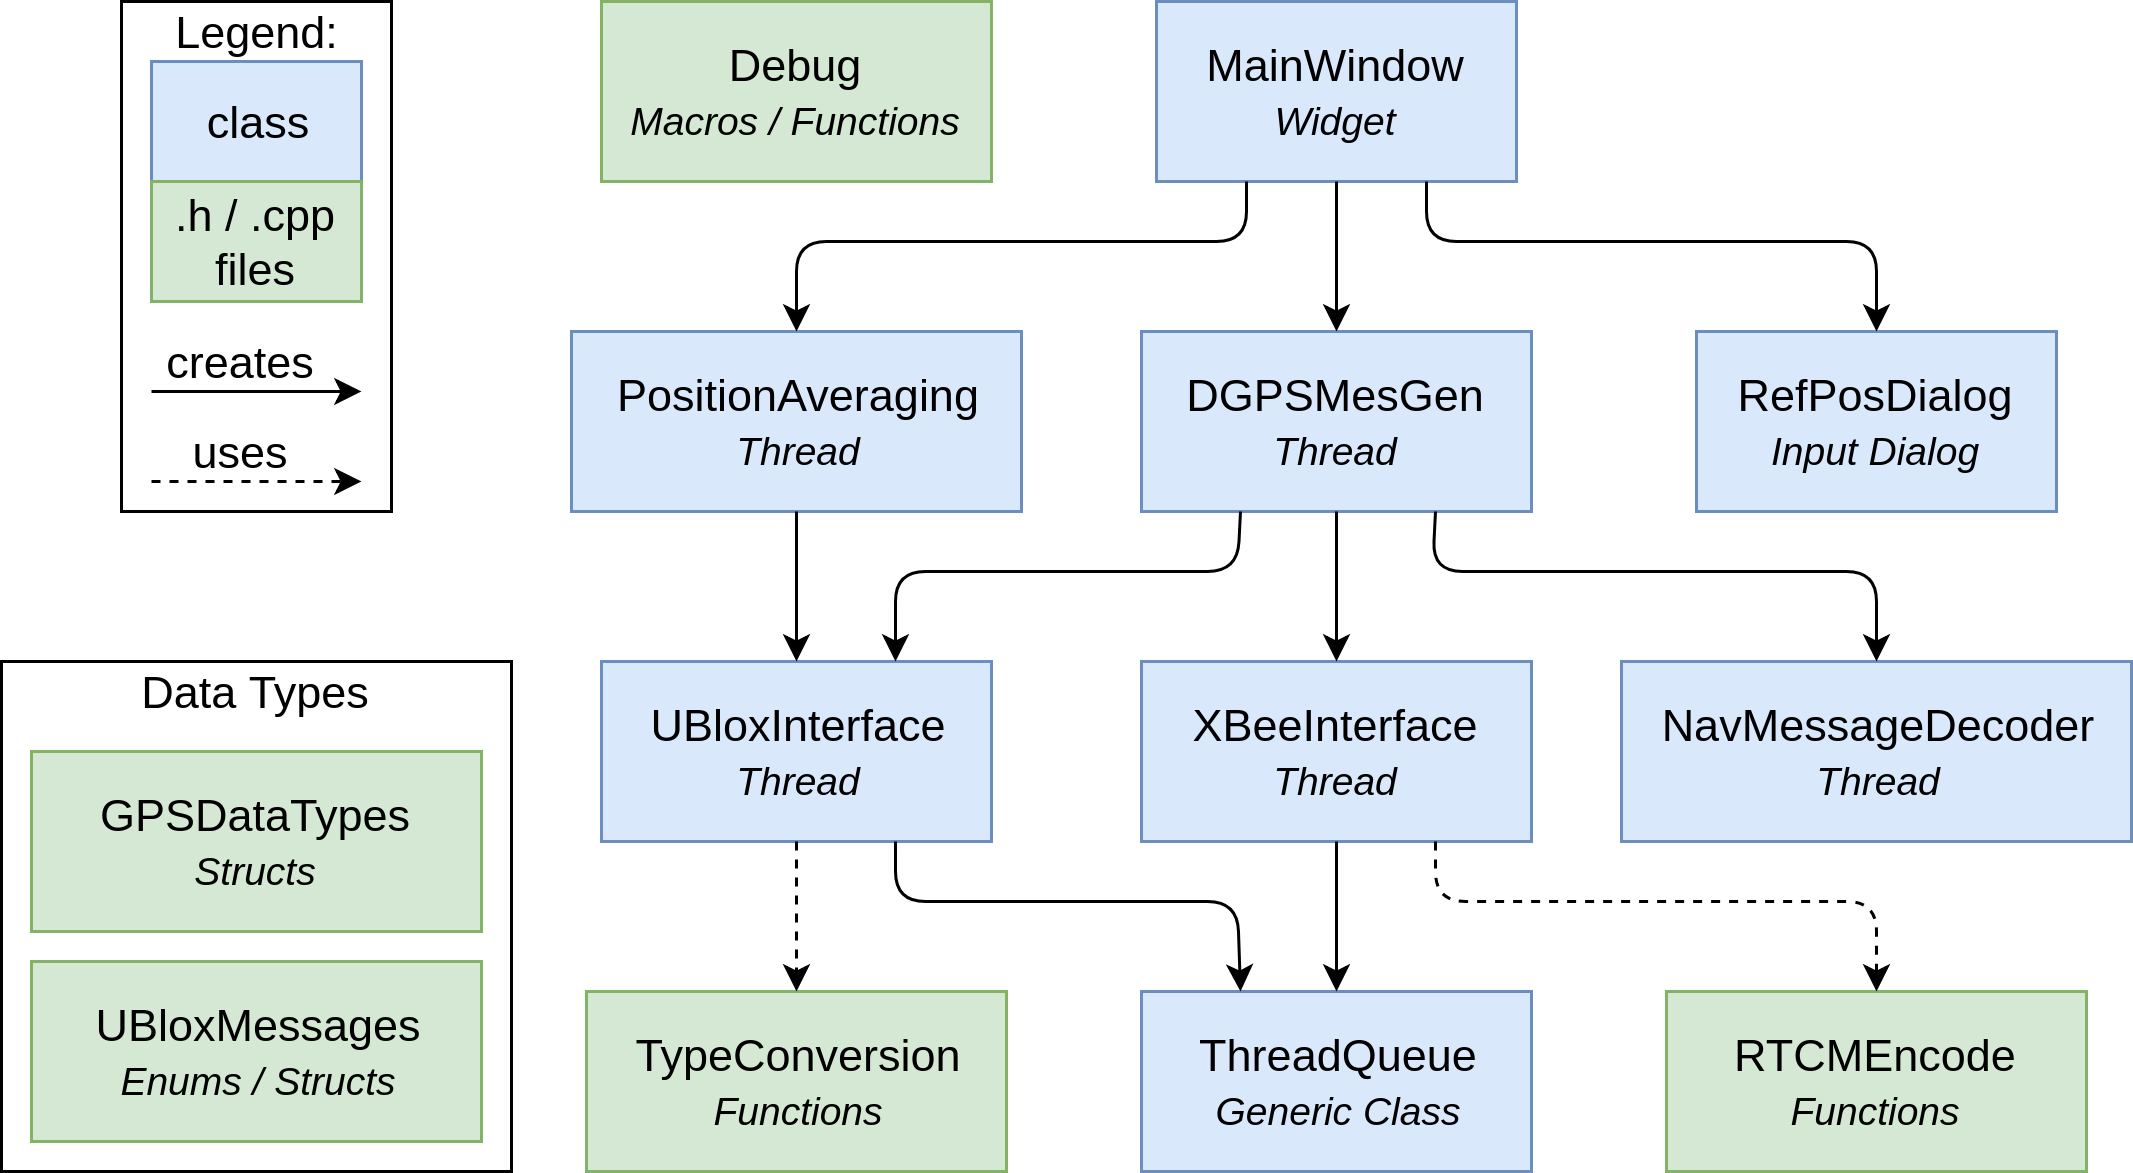
\includegraphics[width=\textwidth]{images/Software_Architecture.png}
 \caption{Software architecture of the DGPS Message Generator}
 \label{fig:software_architecture}
\end{figure}

\subsection{Data Flow}

The data flow graph in figure \ref{fig:data_flow} gives a better overview of the internal functionality of the DGPS Message Generator and how it fits into the ground station infrastructure.
The data stream from the GPS receiver is channeled over a USB port of the laptop to a serial port, from where it can be read from the application.
The UBloxInterface reads the serial stream and extracts the needed messages.
Two ThreadQueues are fed with the messages containing the pseudoranges and the navigation messages.
The Navigation Message Decoder pulls the raw navigation messages from the ThreadQueue and extacts the ephemeris and other satellite data.
If a pseudorange measurement and all needed satellite data is availabel, it is proccessed by the DGPS Message Generator and incorporated in the next correction message.
All the data neede to generate the RTCM message 1 and 3 are forwarded to the XBee Interface.
That is where the data is encoded into the RTCM protocol and then sent out to a XBee application also running on the laptop.
It routes the data over a serial port and USB port to the XBee module.

\begin{figure}[ht]
 \centering
 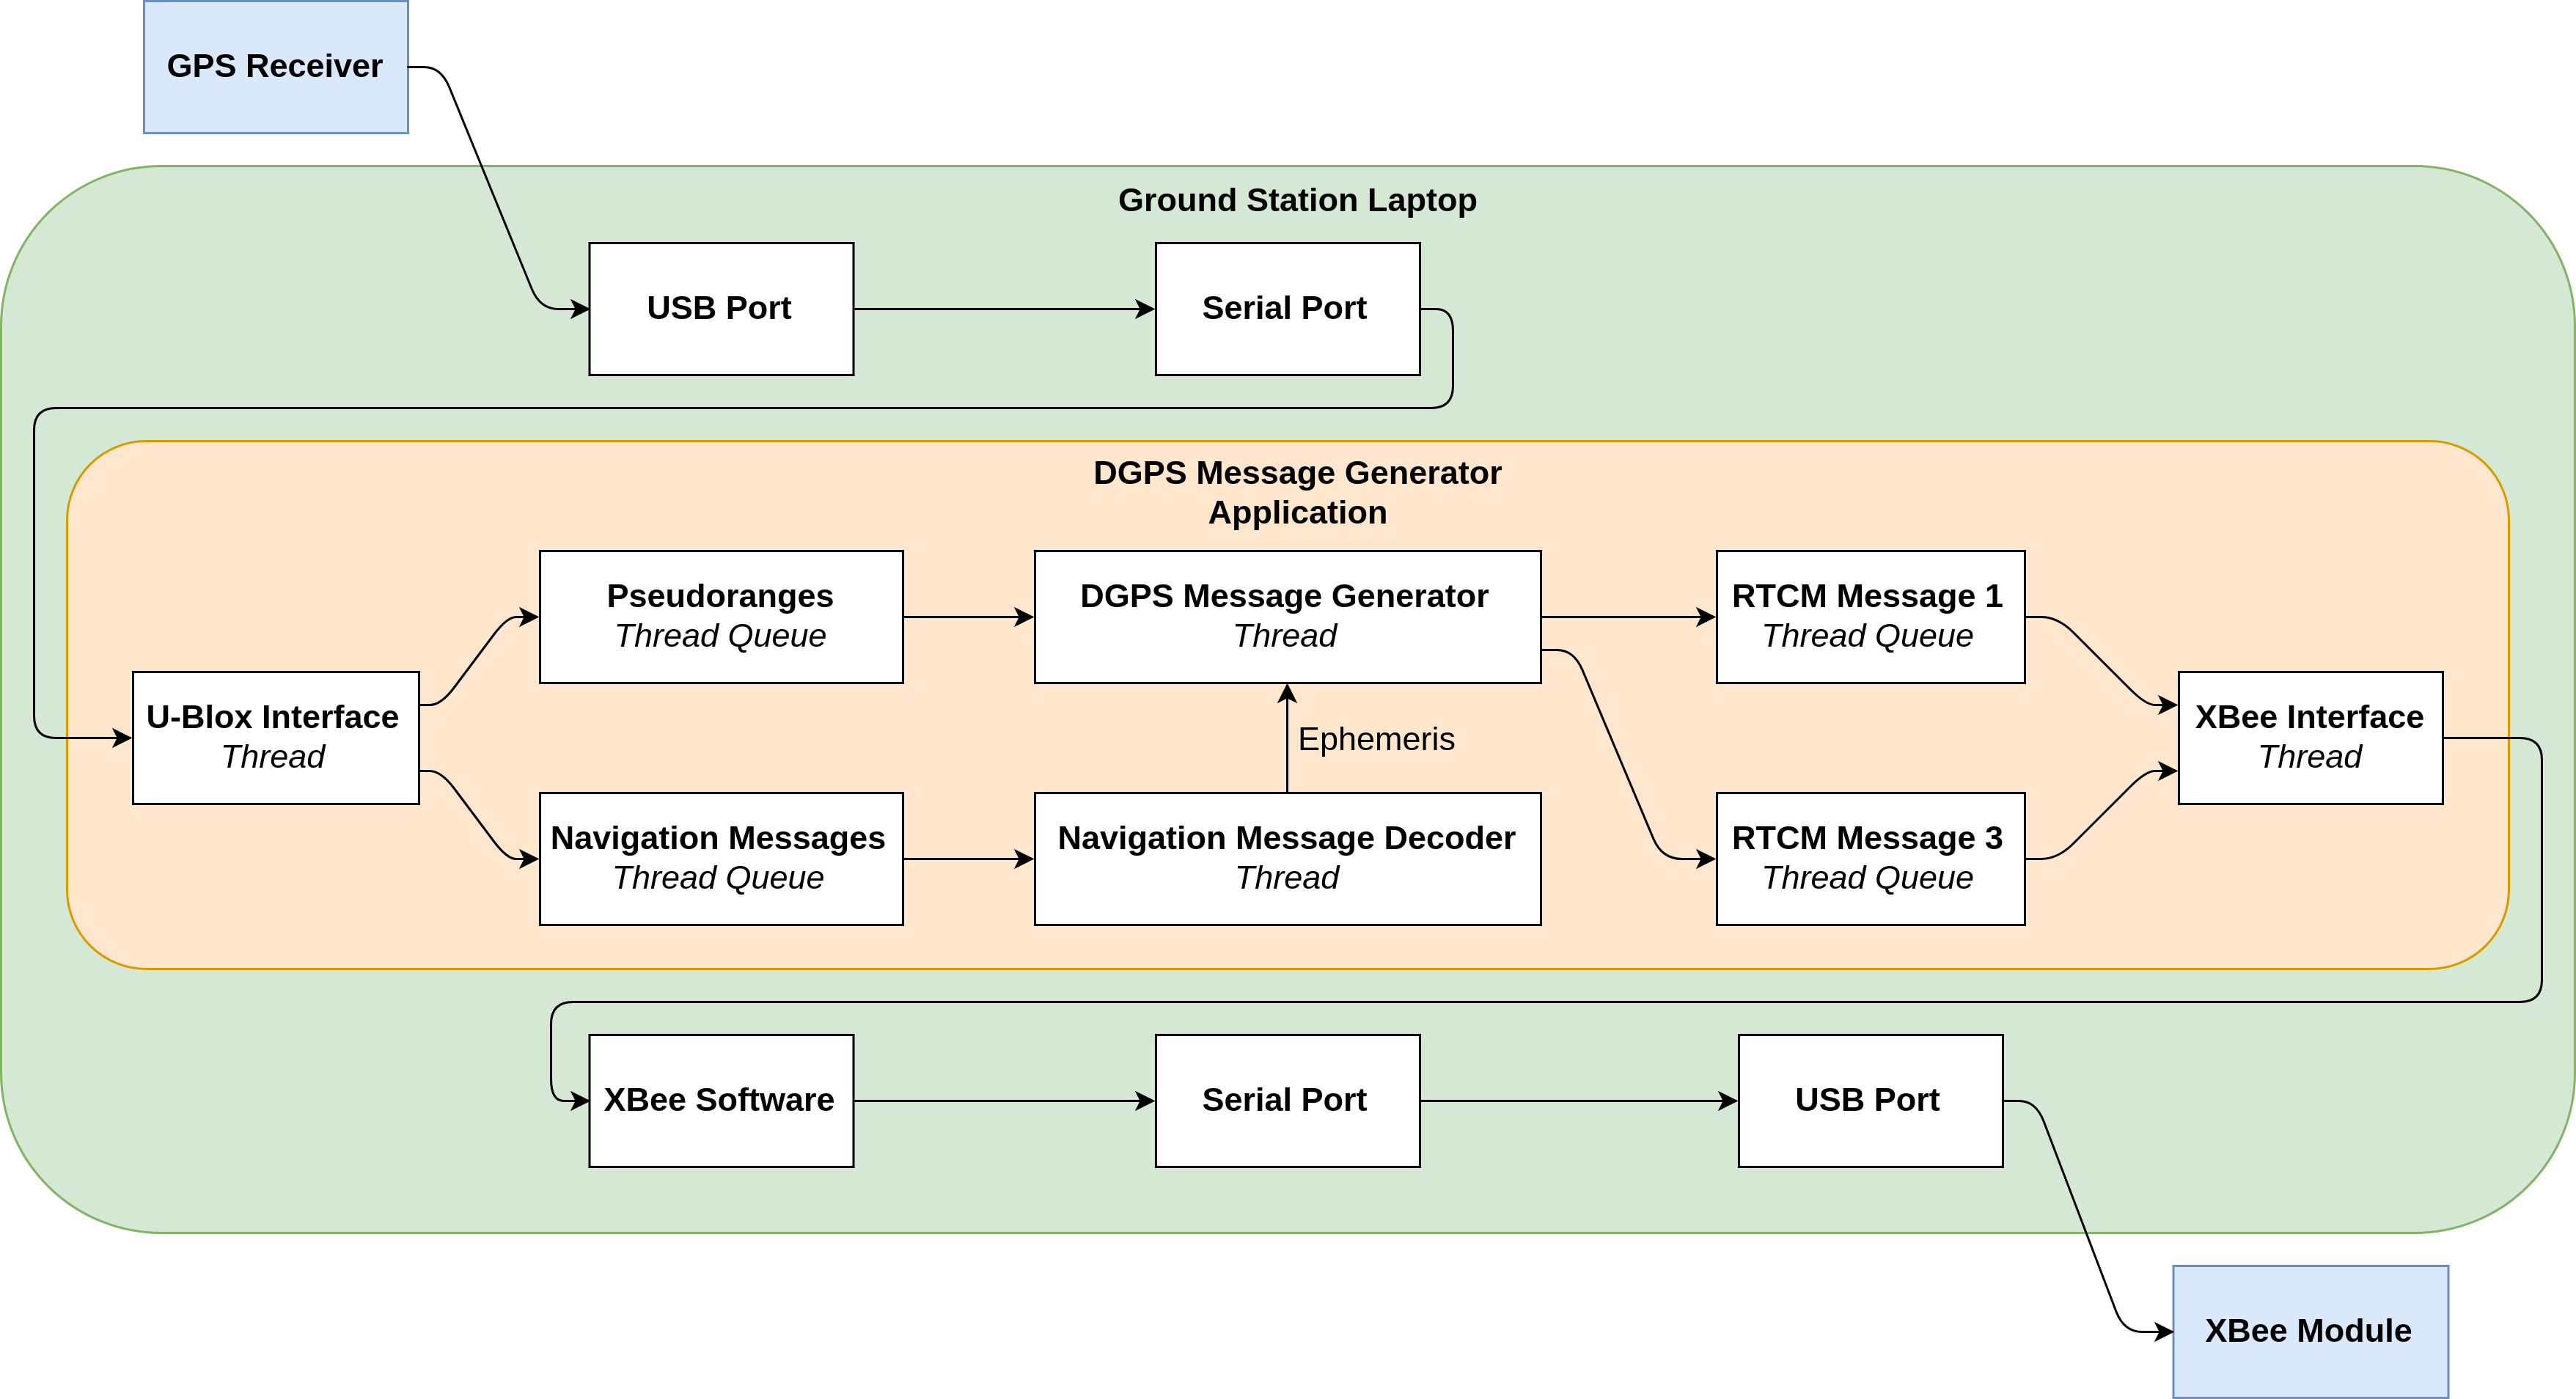
\includegraphics[width=\textwidth]{images/Data_Flow.png}
 \caption{Data flow from the GPS receiver to the XBee module}
 \label{fig:data_flow}
\end{figure}

\subsection{Graphical User Interface}

\begin{minipage}{0.5\textwidth}
 The front end of the application is a graphical interface.
 On the top, it has multiple options to set a reference position.
 It can be set directly over an input dialog, loaded from a file or measured with a connected GPS receiver.
 The position can also be saved to a binary file with the ending .wgs84 for later use.
 The middle section is a sort of command line output.
 All actions made by the user are confiremed there and errors are displayed in red.
 On the bottom, the actual DGPS Message Generator can be started and stopped.
 Input and output port and baud can be specified.
 The output settings are only needed if the external XBee software is bypassed and the RTCM messages are directly sent to a serial port.
\end{minipage}
\hfill
\begin{minipage}{0.45\textwidth}
 \centering
 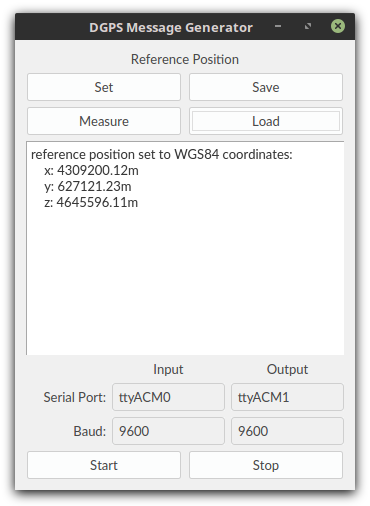
\includegraphics[width=\textwidth]{images/GUI.png}
 \captionof{figure}{Graphical user interface}
 \label{fig:gui}
\end{minipage}

\subsection{U-Blox Interface}

The communication with the GPS receiver takes place over the proprietary UBX messages.
Three messages are needed by the application.
The pseudoranges are transmitted with the UBX-RXM-RAWX message.
The GPS navigation messages are tramsmitted in raw form by the UBX-RXM-SFRBX message.
To be able to measure the reference position, the UBX-NAV-POSECEF message is used.
It has the information of the position estimation in ECEF form.


\subsection{XBee Interface}

\subsection{Navigation Message Decoder}

\subsection{DGPS Message Generator}

\subsection{Position Averaging}

\subsection{Debug}